% !TEX encoding = UTF-8
% !TEX TS-program = pdflatex
% !TEX root = ../tesi.tex
% !TeX spellcheck = it_IT

\chapter{L'azienda}
\begin{figure}[H] 
    \centering
    
\includegraphics[width=0.5\columnwidth]{riskapp-logo} 
    \caption{Logo RiskApp}
    \label{img:riskapp-logo}
\end{figure}
RiskApp è il principale fornitore di tecnologia che possiede una piattaforma di gestione del rischio a tutto tondo per il settore assicurativo. \'E stata concepita per supportare e migliorare le sottoscrizioni, i reclami, le vendite e le decisioni tecniche riguardanti le coperture assicurative: offre quindi dati e analisi dei rischi, consulenza e sviluppo di software per la valutazione dei rischi aziendali.
\medskip
\\RiskApp possiede un algoritmo proprietario che stima il valore del rischio in base a dati raccolti da più fonti ed esprime le perdite economiche che possono derivare da tali rischi, confrontando i risultati con le migliori pratiche del settore. 

\section{Contesto organizzativo e produttivo}
Nell'azienda lavorano come lavoratori autonomi il fondatore, Federico Carturan, il co-fondatore e tecnico informatico Pierpaolo Toniolo e Luca Bizzaro, ingegnere civile. L'ufficio è ubicato a Conselve, all'interno del quale ognuno lavora con la propria macchina. Il \textit{core business} dell'azienda è la fornitura di servizi ad agenti assicurativi, fornendo costantemente nuove funzionalità per la loro già esistente piattaforma RiskApp tramite sviluppo di migliori interfacce software e il miglioramento dell'algoritmo proprietario.

\section{Tecnologie utilizzate}
Il sistema è composto da un \textit{frontend} e un \textit{backend}. Il codice riguardante il \textit{backend} è sviluppato in linguaggio Python 3 e gestito dal web framework \grayname{Django}\cite{site:django}.
\begin{figure}[H] 
    \centering
    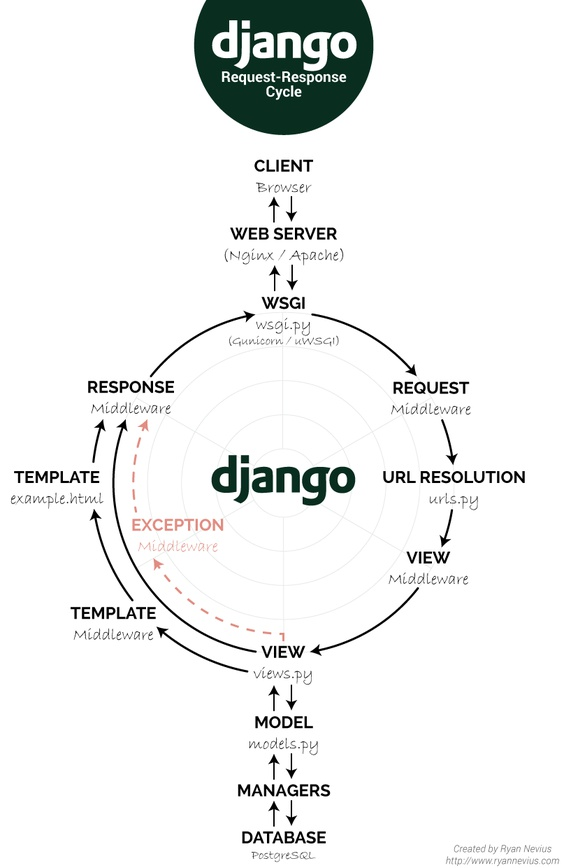
\includegraphics[width=0.5\columnwidth]{django-logo} 
    \caption{Funzionamento Django}
    \label{img:django-logo}
\end{figure}
Il codice riguardante il \textit{frontend} è sviluppato in linguaggio JavaScript, facendo uso del framework \grayname{React}\cite{prod:react} utilizzando come \textit{state container} \grayname{Redux}\cite{prod:redux}. La comunicazione tra \textit{frontend} e \textit{backend} è costituita da chiamate \glslink{rest}{REST} attraverso l'utilizzo di \grayname{Django REST framework}\cite{prod:django-rest-framework}. Per Python viene utilizzato \grayname{PyCharm}\cite{prod:PyCharm}, un \glslink{ide}{IDE} prodotto da JetBrains\textsuperscript{\textcircled{c}} che, oltre ad offrire un assistente "intelligente" per la scrittura di codice e \textit{safe refactoring}, include anche degli strumenti di sviluppo quali \textit{debugging} e \textit{deploying} su GitHub\cite{site:github}. Per quanto riguarda invece JavaScript, viene utilizzato \grayname{IntelliJ IDEA}\cite{prod:IntelliJ}, che offre le stesse funzionalità di \grayname{PyCharm}.

\section{Processi interni}
Il codice è organizzato all'interno di due repository GitHub\cite{site:github} ospitate nel profilo dell'azienda. In particolare, c'è una \textit{repository} per il versionamento del \textit{frontend} e una per quello del \textit{backend}. Lo sviluppo del codice avviene in rami separati per ogni sviluppatore; al compimento delle \textit{features} per una \textit{milestone} viene fatta una \textit{pull request} nel ramo \textit{development}. Quindi, dopo un periodo di test nel server di testing, viene fatta una \textit{pull request} nel ramo master e quindi il \textit{deploy} nell'ambiente di produzione.
\begin{figure}[H] 
    \centering
    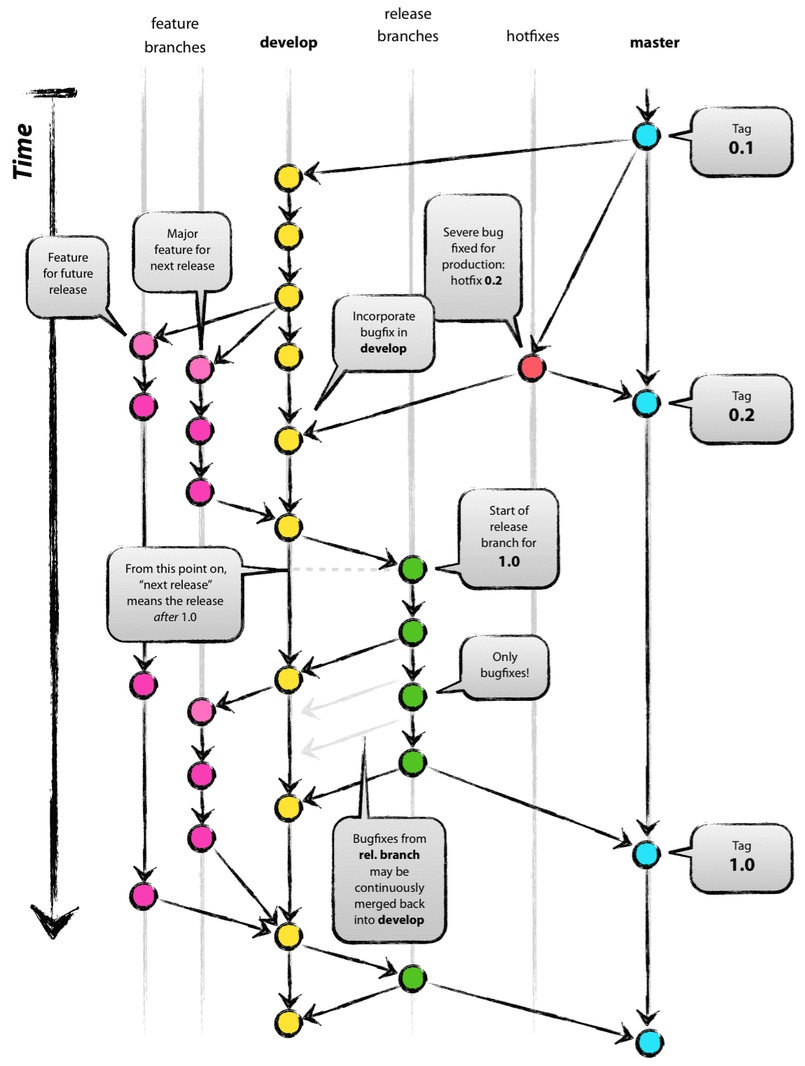
\includegraphics[width=0.5\columnwidth]{git-branches} 
    \caption{Distribuzione del lavoro su rami git}
    \label{img:git-branches}
\end{figure}
Il processo di verifica del codice è automatizzato da script interni che consentono una \textit{continuous integration}. Tali test vengono lanciati ogni volta che avviene un \textit{push} attraverso l'ausilio di \grayname{CircleCI}\cite{prod:circle-ci}, servizio che è integrato con GitHub e che ad ogni \textit{push} in automatico testa la \textit{build} in una macchina virtuale creata appositamente per i test.
\medskip
\\Invece, la gestione delle \textit{milestones} viene fatta attraverso i \textit{projects} di GitHub, in cui vengono fatti convogliare i rispettivi \textit{task} necessari per lo sviluppo delle \textit{features} selezionate. Ogni compito rappresenta un'azione atomica necessaria per l'implementazione della \textit{feature} ed è rappresentata da una \textit{issue} in GitHub. Ogni \textit{issue} viene quindi etichettata per tenere traccia del tipo di azione o priorità che identifica.


\section{Tipologia clientela}
La piattaforma viene principalmente utilizzata da professionisti del rischio, brokers e agenti assicurativi, che la utilizzano per reperire informazioni dettagliate sui i rischi assicurabili e per ricevere un preventivo in maniera istantanea di eventuali polizze.

\section{Innovazione}
RiskApp è una startup concentrata nell’innovazione del settore assicurativo, l’\textit{Insurtech}. Il tutto è nato dalla selezione in Unipol Ideas, il percorso di Open Innovation del Gruppo Unipol: un canale di dialogo e contaminazione con chi fa innovazione in ambiti collegati al core business aziendale. Unipol è tra i soci fondatori della Fondazione ItaliaCamp. Riskapp si è presentata in Expo Milano 2015 al Vivaio delle Idee, lo spazio dedicato all'innovazione ideato e gestito da Padiglione Italia, Ministero delle Politiche Agricole e Forestali e Fondazione ItaliaCamp\cite{site:riskapp-rai}. 
\medskip
\\Nel 2016 Unipol è diventata il primo cliente, inoltre sono state fatti altri programmi di accelerazione in Europa, tra i quali Deloitte Digital Disruptors\cite{site:deloitte-digital-startup} a Lisbona, MundiLab\cite{site:mundi-lab} a Madrid, Fintech Innovation Lab\cite{site:fintech} a Londra che hanno portato alla collaborazione con Società di consulenza quali Deloitte\cite{site:deloitte} e Accenture\cite{site:accenture}, riassicuratori Munich Re\cite{site:munich-re} e Swiss Re\cite{site:swiss-re}, e a nuovi clienti in Europa, come Fidelidade\cite{site:fidelidade} e P\&V\cite{site:pv}.


